\documentclass{beamer}
\usepackage{amsfonts,amsmath,oldgerm}
\usepackage[export]{adjustbox}
\usetheme{sintef}
\newcommand{\testcolor}[1]{\colorbox{#1}{\textcolor{#1}{test}}~\texttt{#1}}
\newcommand{\la}{\langle}
\newcommand{\ra}{\rangle}
\usefonttheme[onlymath]{serif}

%%%%%% COMMANDS LIST
%\vspace{\baselineskip}

%%%%%% TITLE
\titlebackground*{assets/background}
\newcommand{\hrefcol}[2]{\textcolor{cyan}{\href{#1}{#2}}}
\title{Non-perturbative computation of Kaons oscillation amplitudes in Lattice QCD with $N_f = 2+1$ sea quarks and OBC}
%\subtitle{Using \LaTeX\ to prepare slides}
\course{Master's Degree in Theoretical Physics}
\author{\href{mailto:emanuele.rosi@roma1.infn.it}{Emanuele Rosi}}
\IDnumber{1812180}
\date{Academic Year 2022/2023}

%%%%%% DOCUMENT
\begin{document}
\maketitle

\section{Introduction to $K^0$-$\bar K^0$ mixing}

\begin{frame}{Kaons oscillations}
      \framesubtitle{SM oscillations}
      Kaons oscillations in Standard Model (SM) are mediated by Weak Interacitons.
      \begin{itemize}
            \item Two 1-loop order diagrams
      \end{itemize}
      \vspace{\baselineskip}
      \begin{columns}
            \centering
            \begin{column}{0.5\textwidth}
                  \centering
                  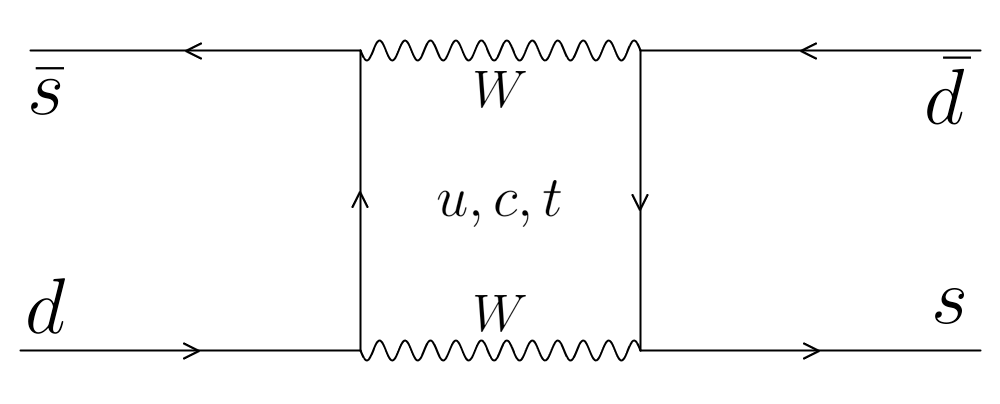
\includegraphics[width=.8\textwidth,right]{assets/kkbar-1.png}
            \end{column}
            \begin{column}{0.5\textwidth}
                  \centering
                  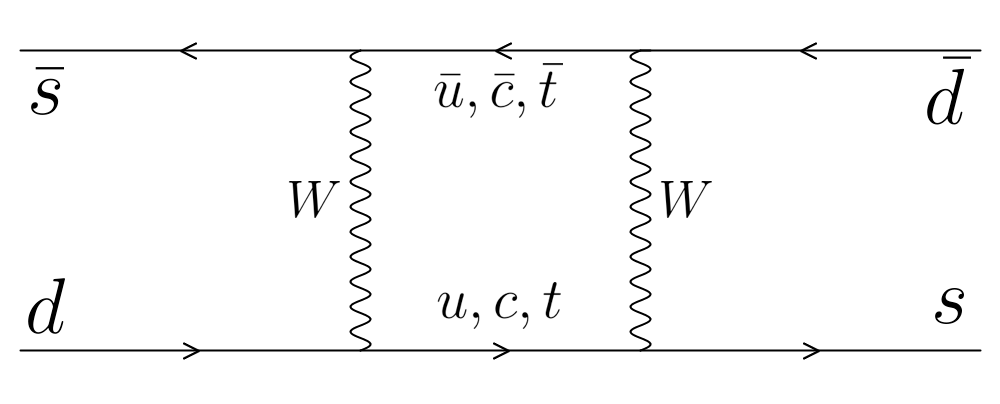
\includegraphics[width=.8\textwidth,left]{assets/kkbar-2.png}
            \end{column}
      \end{columns}
\end{frame}

\begin{frame}{Kaons oscillations}
      \framesubtitle{SM oscillations}
      Kaons oscillations in Standard Model (SM) are mediated by Weak Interacitons.
      \begin{itemize}
            \item Two 1-loop order diagrams
            \item An effective operator arises ($E \ll M_W$):
            \begin{equation*}
                  \la \bar K^0 | \Theta_1 | K^0 \ra \qquad \Theta_1 = \Big[ \bar s^a \gamma_\mu (1-\gamma_5) d^a \Big] \cdot \Big[ \bar s^b \gamma_\mu (1-\gamma_5) d^b \Big]
            \end{equation*}
            \item Perturbative approach (PT) not allowed at energies $\lesssim \Lambda_\text{QCD}$
      \end{itemize}
\end{frame}

\begin{frame}{Kaons oscillations}
      \framesubtitle{SM oscillations}
      Vacuum insertion approximation (VIA):
      \begin{equation*}
            \begin{gathered}
                  \la \bar K^0 | \Big[ \bar s^a \gamma_\mu (1-\gamma_5) d^a \Big] \cdot \Big[ \bar s^b \gamma_\mu (1-\gamma_5) d^b \Big] | K^0 \ra \approx \\
                  \approx \la \bar K^0 | \Big[ \bar s^a \gamma_\mu (1-\gamma_5) d^a \Big] | 0 \ra \la 0 | \Big[ \bar s^b \gamma_\mu (1-\gamma_5) d^b \Big] | K^0 \ra + \\
                  \la \bar K^0 | \Big[ \bar s^a \gamma_\mu (1-\gamma_5) d^b \Big] | 0 \ra \la 0 | \Big[ \bar s^b \gamma_\mu (1-\gamma_5) d^a \Big] | K^0 \ra = \frac{8}{3} F_K^2 m_K^2
            \end{gathered}
      \end{equation*}
      $B_1$ parameter (a.k.a. $B_K$) parametrizes deviation from VIA: $\la \bar K^0 | \Theta_1 | K^0 \ra = \frac{8}{3} B_1 F_K^2 m_K^2$
\end{frame}

\begin{frame}[fragile]{Kaons oscillations}
      \framesubtitle{Oscillations BSM}
      \begin{itemize}
            \item $B_1$ parameter (a.k.a. $B_K$) parametrizes deviation from VIA
            \item Other operators $\{\Theta_i,\tilde\Theta_j\}$ appears in theories beyond the SM (BSM)
            \item They form a complete set of operators of dimension 6, composed by 4 quarks, closed under renormalization procedure
            \item New BSM \emph{bag parameters}:
            \begin{equation*}
                  \la \bar K^0 | \Theta_j^{[+],\text{ren}} (\mu) | K^0 \ra = \xi_j \left(\frac{m_K^2}{m_s(\mu)+m_d(\mu)}\right)^2 f_K^2 B_j(\mu) \qquad j \ge 2
            \end{equation*}
            \item Non perturbative approach $\Longrightarrow$ \emph{path integral}
      \end{itemize}
\end{frame}

\begin{frame}{Purpose of the work}
      \framesubtitle{Introduction}
      \centering
      Non perturbative computation of bare bag parameters $B_i$ on the lattice
      $$\downarrow$$
      Coordinated Lattice Simulations (CLS) gauge configurations with $N_f = 2+1 $\\ sea quarks and open boundary conditions (OBC) in time direction
\end{frame}

\section{Lattice regularizations of QFTs}

\begin{frame}{Lattice regularizations of QFTs}
      Regularizations ingredients:
      \begin{itemize}
            \item Lattice space $\Lambda$ of dimension $L \times L \times L \times T$
            \item Lattice spacing $a$: $L = a\cdot N_L$, $T = a\cdot N_T$
            \item Action discretization:
            \begin{equation*}
                  S^\text{lat}[a;\tilde\phi_1,\dots,\tilde\phi_{N_\text{fields}}] \hspace*{1mm} \xrightarrow{\hspace*{3mm} a \rightarrow 0\hspace*{3mm}} \hspace*{1mm} S^\text{cont}[\phi_1,\dots,\phi_{N_\text{fields}}]
            \end{equation*}
            \item Troubles: finite volume effects \& lattice spacing effects
            \item $O(a^n)$-improvement:  $S^\text{lat}(a) = S^\text{cont} + o(a^{n})$
      \end{itemize}
\end{frame}

\begin{frame}{Action regularizations}
      Many regularizations have been developed
      \vspace{\baselineskip}
      \begin{columns}
            \begin{column}{0.45\textwidth}
                  Gauge actions:
                  \begin{itemize}
                        \item Link variables $$U_\mu (x) = \text{exp}\left(i\int_x^{x+a\hat\mu} A_\nu(\omega)d\omega^\nu \right)$$
                        \item Wilson loops are gauge invariant 
                        \item Plaquette, tree level improved Symanzik, Luscher Weisz
                  \end{itemize}
            \end{column}
            \begin{column}{0.45\textwidth}
                  Fermion actions:
                  \begin{itemize}
                        \item Wilson-Dirac action\\Wilson term $r \in [-1,1]$
                        \item Sheikholeslami-Wohlert term: $$ D^W_{xy} \longmapsto D^W_{xy} + c_{SW} \frac{ia}{4}\sigma_{\mu\nu}\hat F_{\mu\nu} (x) \delta_{xy} $$
                        \item Osterwalder-Seiler action\\(twist transformation)
                  \end{itemize}
            \end{column}
      \end{columns}
\end{frame}

\begin{frame}{Simulation troubles}
      \begin{itemize}
            \item Gauge configuration exhibit long autocorrelation times as $a\rightarrow 0$
            \item Zero modes of $D^W_{xy}$ make the sea quarks simulation inefficient 
            \item[]\begin{center}
                  $\Downarrow$\\
                  {\bf Open boundary conditions (OBC) in time direction}
                  \end{center}
            \begin{equation*}
                  \begin{gathered}
                      F_{0i}(\vec x, x_4=0) = F_{0i}(\vec x, x_4=T) = 0 \qquad \forall i = 1,2,3 \\
                      \begin{aligned}
                          & P_+ \psi (\vec x, 0) = P_- \psi (\vec x, T) = 0 \\
                          & \bar\psi (\vec x, 0) P_- = \bar\psi (\vec x, T) P_+ = 0 
                      \end{aligned}
                      \quad\quad P_{\pm} = \frac{1}{2}\left(\mathbb{I} \pm \gamma_5 \right)
                  \end{gathered}
            \end{equation*}
            \item Restoration of connection of gauge fields space
            \item IR protection against zero modes
      \end{itemize}
\end{frame}

\begin{frame}{Sea actions}
      \begin{itemize}%[<+->]
            \item Gauge action: Luscher-Weisz action
            $$ S_G[U] = \frac{1}{g_0^2}\left(\frac{5}{3}\sum_{\{P\}} \text{Tr}\left(\mathbb{I} - U_P \right) - \frac{1}{12}\sum_{\{R\}}\text{Tr}\left( \mathbb{I}-U_R \right) \right)$$
            \item Sea quarks: Dirac-Wilson + SW term
            $$ S^\text{sea}[U,f,\bar f] = \sum_{q=1}^3 \sum_{x} \bar f_q (x) \left[ D^{WD}(r_q) + \frac{ia}{4}c_{SW}\sigma_{\mu\nu}\hat{F}_{\mu\nu} + m^\text{bare}_q \right] f_q (x) $$
      \end{itemize}
\end{frame}

\begin{frame}{Valence actions}
      \begin{itemize}
            \item Valence quarks: Osterwalder-Seiler at Maximal twist + SW term
            \begin{equation*}
                  S^\text{val}[U,\psi,\bar\psi] = a^4 \sum_q \sum_x \bar \psi_q (x) \left[ D^{WD}(r_q) + \frac{ia}{4}c_{SW}\sigma_{\mu\nu}\hat{F}_{\mu\nu} + m^\text{cr} + i \gamma_5 \mu_q^\text{bare} \right] \psi_q (x)
            \end{equation*}
      \end{itemize}
      \begin{columns}
            \begin{column}{0.5\textwidth}
                  \begin{itemize}
                        \item Flavours: $d,d',s,s'$ with\\ $\mu_s = \mu_{s'}$, $\mu_d=-\mu_{d'}$\\equiv. $r_d = r_s = r_{s'} = -r_{d'} = \pm 1$
                        \vspace{\baselineskip}
                        \item Bosonic ghosts $\{\phi_q, \bar \phi_q\}$ to cancel valence quarks determinant
                  \end{itemize}
            \end{column}
            \begin{column}{0.45\textwidth}
                  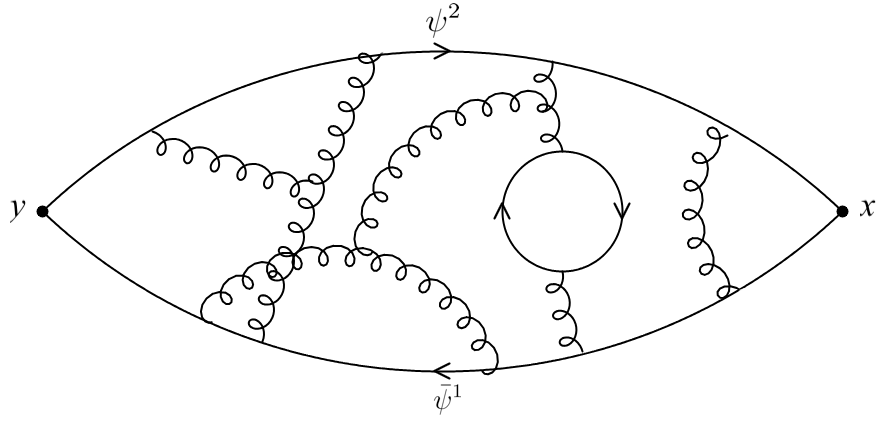
\includegraphics[width=\textwidth]{assets/confinement_bis.png}
            \end{column}
      \end{columns}
\end{frame}

\section{Mixing operators on the lattice}

\begin{frame}{Frezzotti \& Rossi Strategy}
      Why do we need flavor replicas $d,d',s,s'$ ? Because of R. Frezzotti \& G. Rossi strategy!
      \vspace{\baselineskip}
      \newline
      A rather long chain of transformations:
      \begin{center}
            Operators $\{\Theta_i^{[\pm]}\}$ in continuum QCD $\xrightarrow{ \text{basis change} }$ Operators $\{Q_i^{[\pm]}\}$ in continuum QCD\\
            \vspace{\baselineskip}
            $\xrightarrow{ \text{flavour replicas} }$ P.E. operators $\{O_{i,[+]}^\text{phys}\}$ $\xrightarrow{ \text{maximal twist} }$ P.E. operators $\{O_{i,[+]}^\text{tw}\}$
      \end{center}
\end{frame}

\begin{frame}{Frezzotti \& Rossi Strategy}     
      Flavour replicas and twist: a simple example\\
      \begin{equation*}
            \begin{split}
                  & \bar{K}^{0'}=\bar s' \gamma_5 d' = \bar \chi^3 \gamma_5 \chi^4 \\
                  & \bar{K}^{0} =\bar s\gamma_5 d = \bar \chi^1 \gamma_5 \chi^2
            \end{split}
            \quad \text{Maximal Twist } \chi^i = e^{i\gamma_5 r_i \frac{\pi}{4}}\psi^i \qquad
            \begin{split}
                  & \bar{K}^{0'}=\bar \psi^3 \gamma_5 \psi^4 \\
                  & \bar{K}^{0} = i \bar \psi^1 \psi^2
            \end{split}
      \end{equation*}
      Similar transformations act on operators $O_{i[+]}$ and map PE operators in PO ones.
      \vspace{\baselineskip}
      \newline
      {\bf Achievements:}\newline
      Specific regularization of the valence quarks in order to obtain:
      \begin{itemize}%[<+->]
            \item $O(a)$-improved mixing amplitudes w/o the need for W.A.
            \item Absence of wrong chirality mixing between $\{O_i^{[+]}\}$ and $\{O_i^{[-]}\}$
            \item Blocks like renormalization matrix $[Z_{ij}]$ for parity odd operators
      \end{itemize}
\end{frame}

\begin{frame}{Asymptotic behaviours}
      Two and three points correlators:
      \begin{equation*}
            \begin{split}
                  & C_i (x_4,y_4,z_4) = \sum_{\vec x,\vec y,\vec z}     \la \Omega | T \left\{ \bar K^{0'}(x)O_{i[+]}(y)\bar K^{0} (z) \right\} | \Omega \ra \\
                  & G_{34} (x_4,y_4) = \sum_{\vec x,\vec y}             \la \Omega | T \left\{ \bar K^{0'} (x) K^{0'} (y)              \right\} | \Omega \ra \\
                  & G_{12} (x_4,y_4) = \sum_{\vec x,\vec y}             \la \Omega | T \left\{ \bar K^{0} (x) K^{0} (y)                \right\} | \Omega \ra \\
                  & X_{34} (x_4,y_4) = \sum_{\vec x,\vec y}             \la \Omega | T \left\{ \bar A_{4}' (x) K^{0'} (y)              \right\} | \Omega \ra \\
                  & X_{12} (x_4,y_4) = \sum_{\vec x,\vec y}             \la \Omega | T \left\{ \bar A_{4} (x) K^{0} (y)                \right\} | \Omega \ra \\                  
            \end{split}
      \end{equation*}
\end{frame}

\begin{frame}{Asymptotic behaviours}
      Asymptotic behaviours for $x_4 \gg y_4 \gg z_4$:
      \begin{equation*}
            \begin{split}
                  & C_i (x_4,y_4,z_4) \approx \sum_{\vec{y}} \la \Omega | \bar K^{0'} | \bar K^{0'} \ra \la \bar K^{0'} | O_{i[+]} | K^{0} \ra \la K^{0} | \bar K^{0} | \Omega \ra e^{-m_{K'} (x_4-y_4)-m_K (y_4-z_4)}\\
                  & G_{34} (x_4,y_4)  \approx \sum_{\vec{y}} \la \Omega | \bar K^{0'} | \bar K^{0'} \ra \la \bar K^{0'} | K^{0'}                    | \Omega \ra e^{-m_{K'} (x_4-y_4)} \\
                  & G_{12} (x_4,y_4)  \approx \sum_{\vec{y}} \la \Omega | \bar K^{0}  | \bar K^{0}  \ra \la \bar K^{0}  | K^{0}                     | \Omega \ra e^{-m_K (x_4-y_4)}    \\
                  & X_{34} (x_4,y_4)  \approx \sum_{\vec{y}} \la \Omega | \bar A_{4}' | \bar K^{0'} \ra \la \bar K^{0'} | K^{0'}                    | \Omega \ra e^{-m_{K'} (x_4-y_4)} \\
                  & X_{12} (x_4,y_4)  \approx \sum_{\vec{y}} \la \Omega | \bar A_{4}  | \bar K^{0}  \ra \la \bar K^{0}  | K^{0}                     | \Omega \ra e^{-m_K (x_4-y_4)}    \\                  
            \end{split}
      \end{equation*}
\end{frame}

\begin{frame}{Asymptotic behaviours}
      Bag parameters are recovered in continuum limit $a \rightarrow 0$ for $x_4 \gg y_4 \gg z_4$:
      \begin{equation*}
            \begin{split}
                  & \mathcal{B}_1 (a) \approx \frac{3}{8}\cdot\frac{C_1(x_4,y_4,z_4)}{X_{34}(x_4,y_4)X_{12}(y_4,z_4)} \xrightarrow{ \quad a \rightarrow 0 \quad } B_K \\
                  & \mathcal{B}_i (a) \approx \frac{1}{\xi_i}\cdot\frac{\Lambda_{ij}C_j(x_4,y_4,z_4)}{A_{34}(x_4,y_4)A_{12}(y_4,z_4)} \xrightarrow{ \quad a \rightarrow 0 \quad } B_i
            \end{split}
      \end{equation*}
      $\Rightarrow$ Need for 2 and 3 points correlation functions computation
\end{frame}

\section{Simulation Program}

\begin{frame}{Noise spinors method}
      \begin{columns}
            \begin{column}{0.65\textwidth}
                  Mesonic sources in $x_4$ and $z_4$ are simulated through noise spinors $\eta^{(x_4)}$ and $\eta^{(z_4)}$:
                  \begin{itemize}%[<+->]
                        \item Two sets of $N_n$ spinors randomly generated
                        \item The sums $\sum_{\vec{x}}$ and $\sum_{\vec{z}}$ automatically implied when calculating the average over $\eta$s
                        \item Computational advantage
                        \item Different Wick contractions are obtained by multiplying propagators from sources with Dirac matrices
                  \end{itemize}
            \end{column}
            \begin{column}{0.35\textwidth}
                  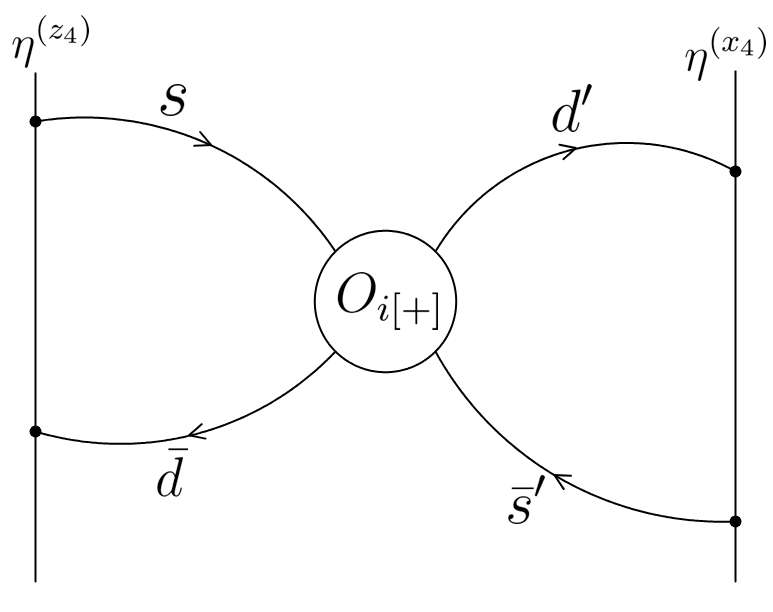
\includegraphics[width=\textwidth]{assets/eta-spinors.png}
            \end{column}
      \end{columns}
\end{frame}


\begin{frame}{Noise spinors method}
      Two types of diagrams:
      \begin{center}
            \begin{figure}
                  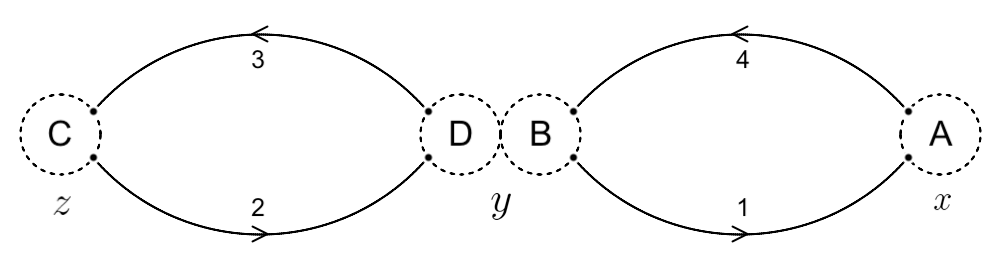
\includegraphics[width=0.45\textwidth]{../thesis-tex/imgs-MSc-thesis/Wick_stochastic_disc.png}
                  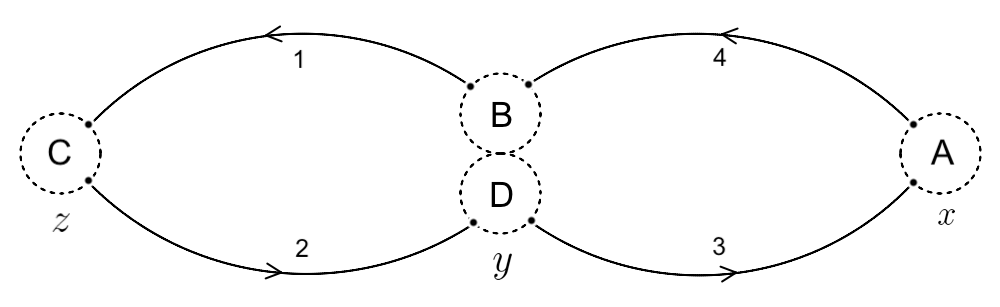
\includegraphics[width=0.4\textwidth]{../thesis-tex/imgs-MSc-thesis/Wick_stochastic_conn.png}
            \end{figure}
      \end{center}
      Two types of noise spinors contractions:
      \begin{equation*}
            \begin{gathered}
                  G_d =   \sum_{\vec y} \left\langle \left\langle \left(\gamma_5\xi^{(3,-)}_{1,A} (y) \right)^\dag \Gamma_B \zeta^{(4,+)}_1 (y) \cdot \left(\gamma_5\xi^{(1,-)}_{C,2} (y) \right)^\dag \Gamma_D \zeta^{(2,+)}_2 (y) \right\rangle^\text{noise} \right\rangle^{\text{sea}} \\
                  G_c = - \sum_{\vec y} \left\langle \left\langle \left(\gamma_5\xi^{(3,-)}_{1,A} (y) \right)^\dag \Gamma_D \zeta^{(2,+)}_2 (y) \cdot \left(\gamma_5\xi^{(1,-)}_{C,2} (y) \right)^\dag \Gamma_B \zeta^{(4,+)}_1 (y) \right\rangle^\text{noise} \right\rangle^{\text{sea}}
            \end{gathered}
      \end{equation*}
\end{frame}

\begin{frame}{Simulation program tests}
      Tests:
      \begin{itemize}
            \item Gauge invariance test
            \item Gauge invariance + investigation about $N_n$
            \item Test on \emph{Tree level improved Symanzik action}, quenched approximation
            \item Test on \emph{Plaquette gauge action}, quenched approximation
      \end{itemize}
\end{frame}

\begin{frame}{Test \#1: Gauge invariance}
      Gauge transformed propagators:\newline
      \begin{equation*}
            \left(S^{(f)}(y, x)[\Omega U \Omega^\dagger]\right)^{b,a}_{\beta,\alpha} = \Omega (y)^{b,c} \left(S^{(f)}(y,x)[U]\right)^{c,d}_{\beta,\alpha} \Omega^\dagger (x)^{d,a}
      \end{equation*}
      \begin{itemize}
            \item Equation tested in three points integrated correlators $C_{i,[+]}$
            \item Link variables $U_\mu (x)$ are randomly generated and then transformed
            \item Pointlike sources instead of random spinors $\eta$
      \end{itemize}
\end{frame}

\begin{frame}{Test \#2: Gauge invariance and investigation about $N_n$}
      \begin{columns}
            \begin{column}{0.43\textwidth}
                  \begin{itemize}
                        \item Equation tested in three points integrated correlators $C_{i,[+]}$
                        \item Link variables $U_\mu (x)$ are randomly generated and then transformed
                        \item Use of random spinors $\eta$
                        \item Different number of $N_n$ were tested. Estimator:
                        \begin{equation*}
                              \varepsilon(N_n) = \frac{1}{N_T-2}\sum_{y_4}\left(\frac{|C(y_4)-\tilde C(y_4)|}{C(y_4)+\tilde C(y_4)}\right)
                        \end{equation*}
                  \end{itemize}
            \end{column}
            \begin{column}{0.57\textwidth}
                  \begin{center}
                        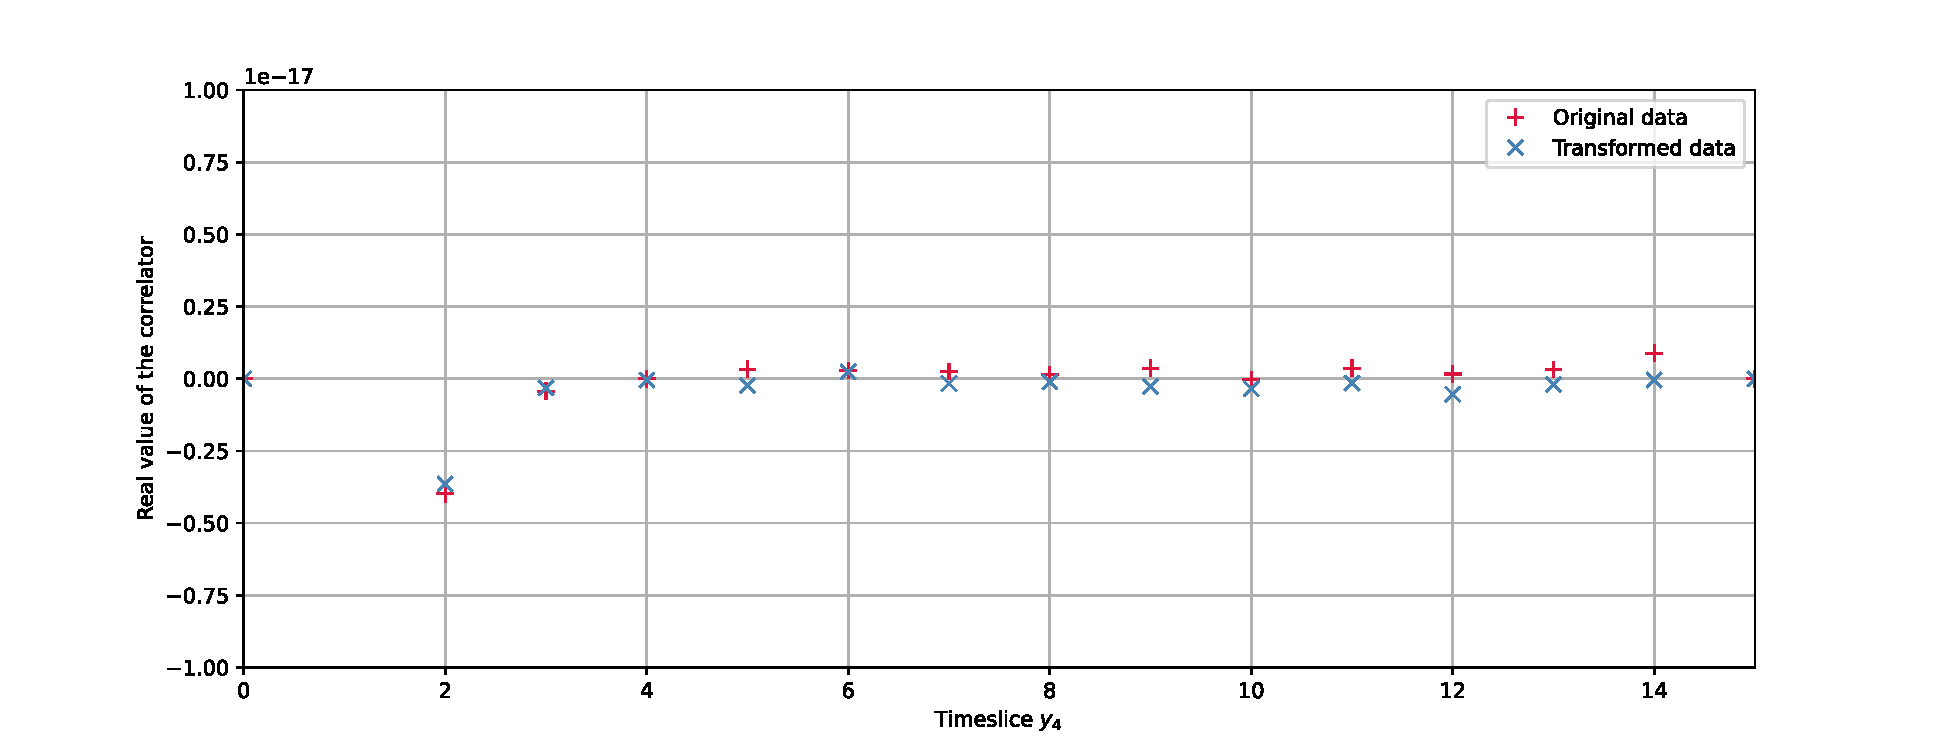
\includegraphics[width=.8\textwidth]{../thesis-tex/imgs-MSc-thesis/check2-20.pdf}\\
                        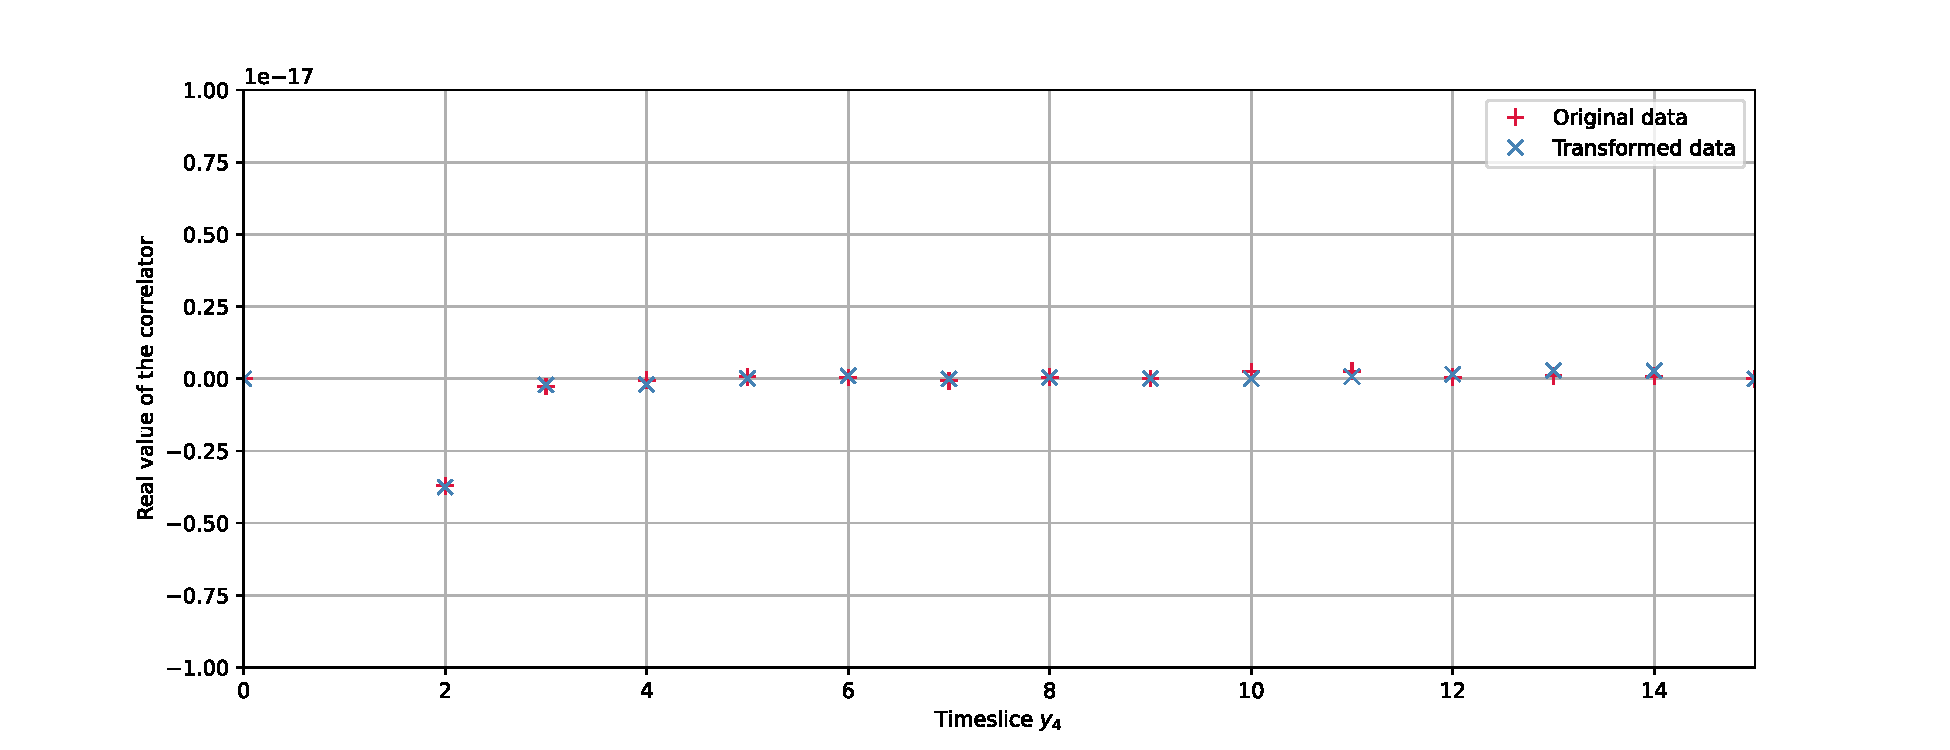
\includegraphics[width=.8\textwidth]{../thesis-tex/imgs-MSc-thesis/check2-100.pdf}
                  \end{center}
            \end{column}
      \end{columns}
\end{frame}

\begin{frame}{Test \#3: tree level improved Symanzik}
      54 Gauge configurations - tree level improved Symanzik action\newline
      16x16x16x32 lattice, $\beta = 6.0$, OBCs, unphysical parameters.
      \begin{columns}
            \begin{column}{.5\textwidth}
                  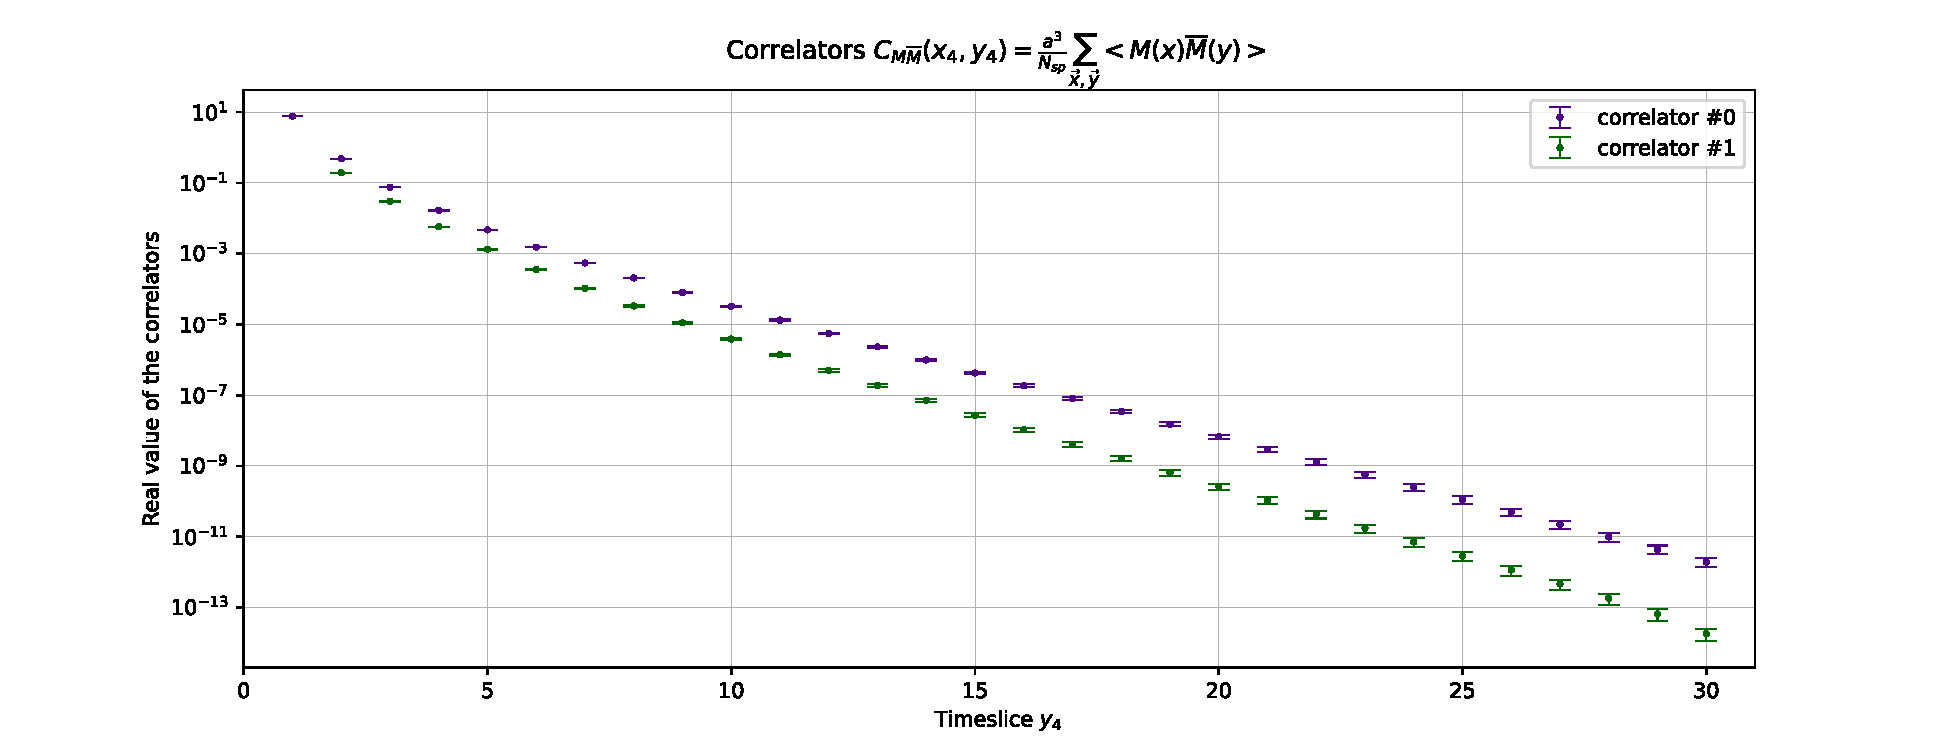
\includegraphics[width=\textwidth]{../thesis-tex/imgs-MSc-thesis/pureYM-2pts.pdf}
                  $$G_{12}(x_4,y_4), G_{34}(x_4,y_4)$$
            \end{column}
            \begin{column}{.5\textwidth}
                  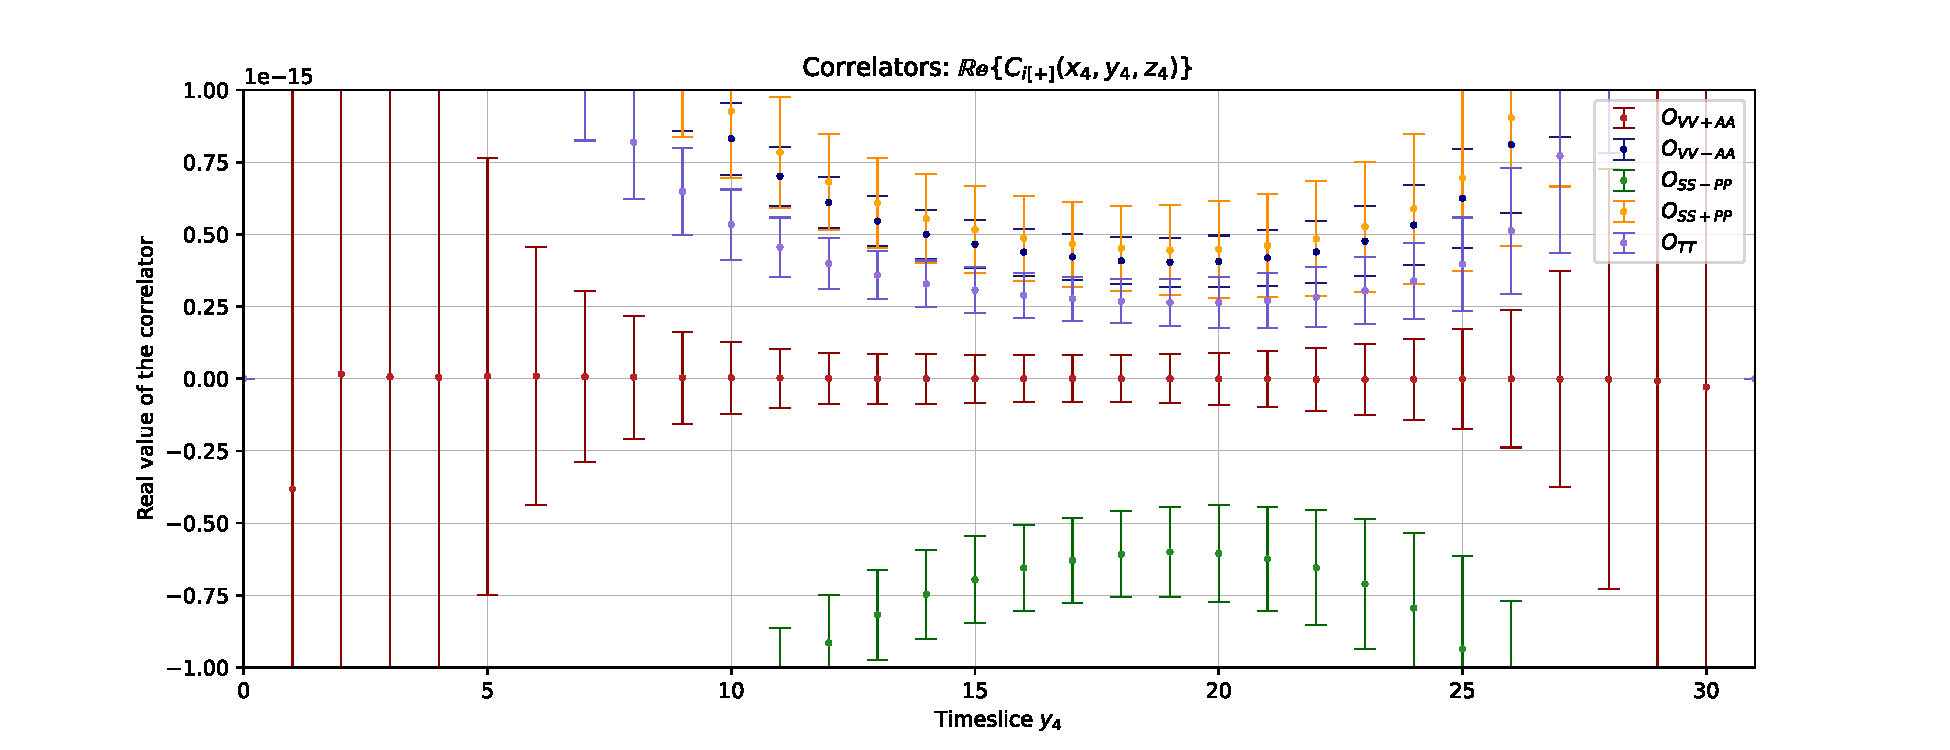
\includegraphics[width=\textwidth]{../thesis-tex/imgs-MSc-thesis/pureYM-3pts.pdf}
                  $$C_{i[+]}(14a,y_4,a)$$
            \end{column}
      \end{columns}
      \vspace{\baselineskip}
      \centering{$M \ne M_\text{crit} \Rightarrow$ not maximal twist.}
\end{frame}

\begin{frame}{Test \#4: Plaquette gauge action}
      37 Gauge configurations - plaquette gauge action\newline
      16x16x16x32 lattice, $\beta = 6.0$, OBCs, maximal twist achieved
      \begin{columns}
            \begin{column}{.5\textwidth}
                  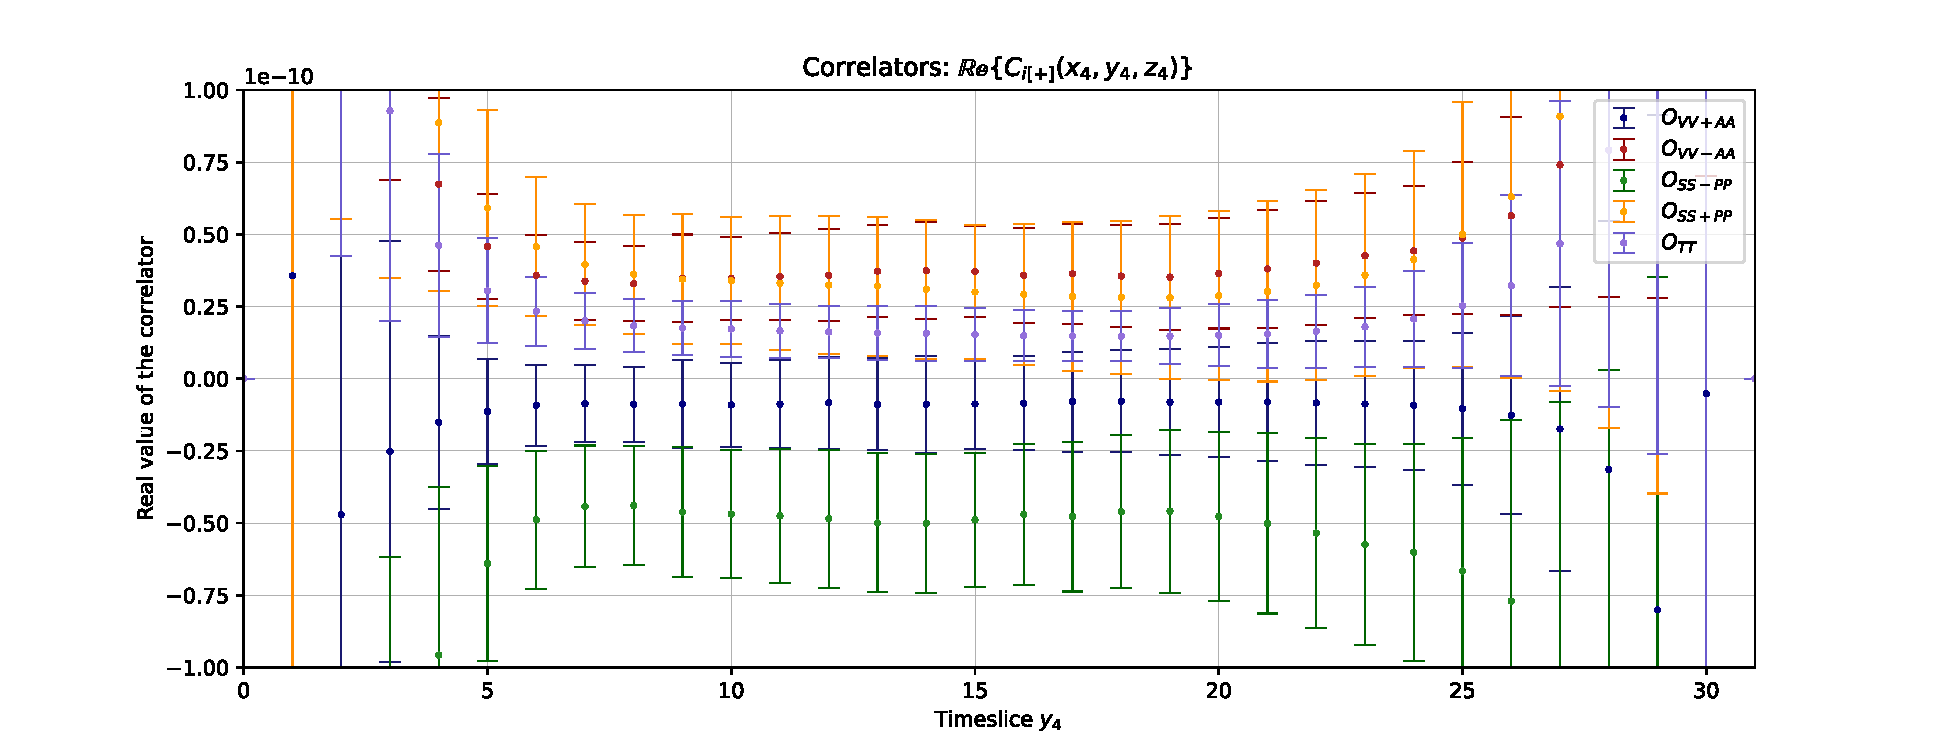
\includegraphics[width=\textwidth]{../thesis-tex/imgs-MSc-thesis/plaq-3pts.pdf}
                  $$C_{i[+]}(14a,y_4,a)$$
            \end{column}
            \begin{column}{.5\textwidth}
                  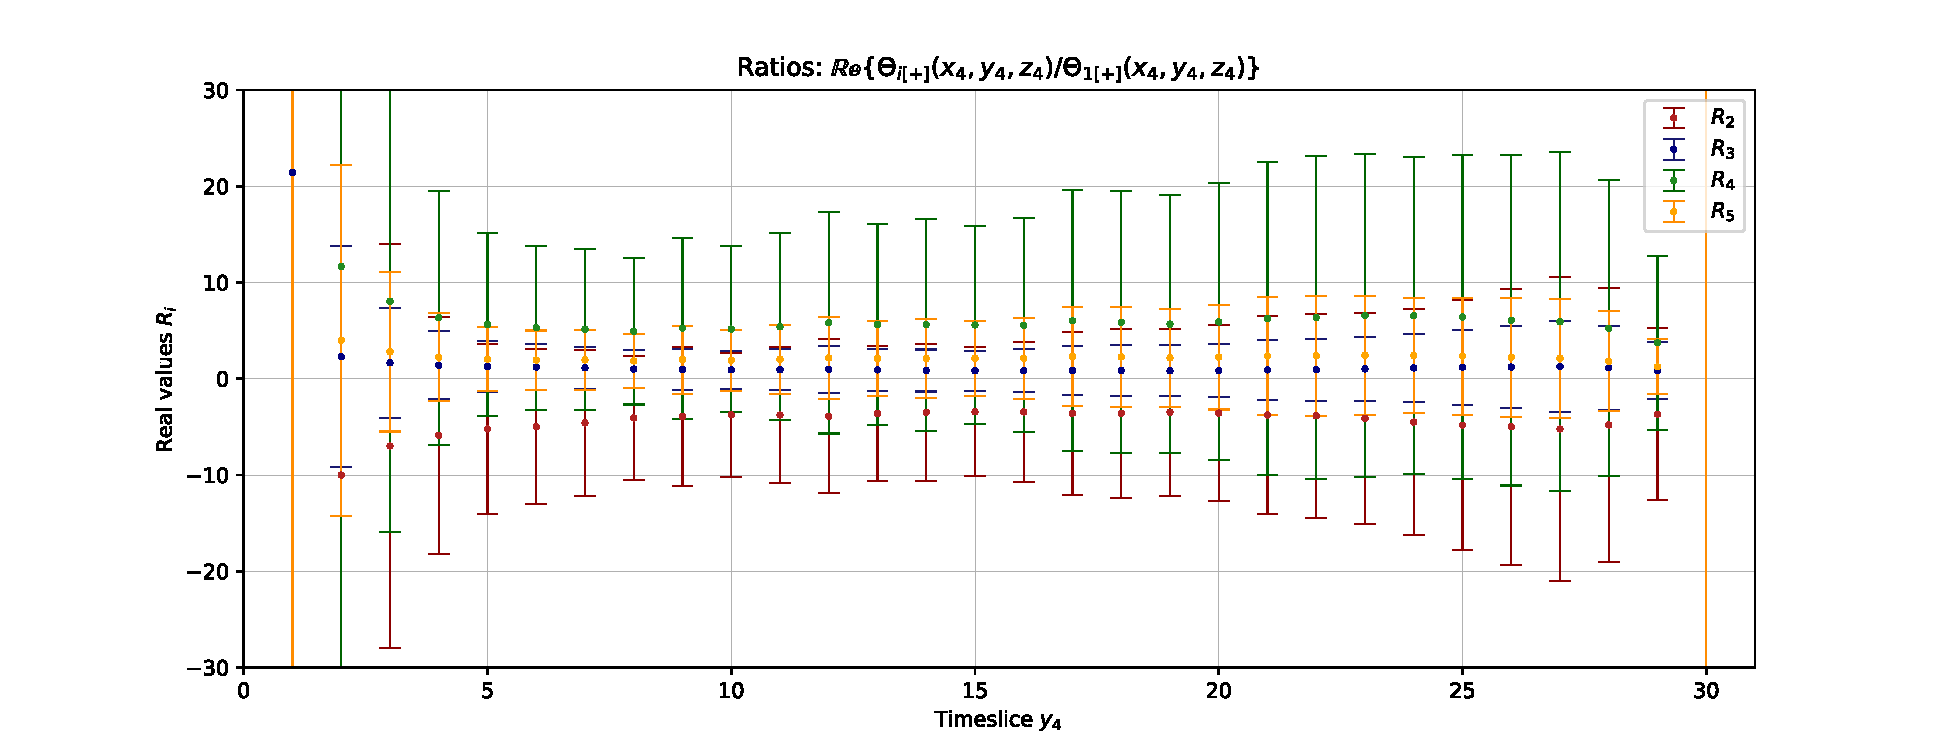
\includegraphics[width=\textwidth]{../thesis-tex/imgs-MSc-thesis/ratios.pdf}
                  $$\mathcal{R}_i (14a,y_4,a) = \Lambda_{ij}\frac{C_{i[+]}(14a,y_4,a)}{C_{1[+]}(14a,y_4,a)}$$
            \end{column}
      \end{columns}
\end{frame}

\begin{frame}{Future developments}
      \begin{itemize}
            \item tests on faithful Gauge configurations with known parameters ($M_\text{crit}, c_{SW}, \mu_is$)
            \item runs over the $N_f = 2+1$ CLS sea ensembles (many values of $a$)
            \item data analysis 
            \item continuum limit extrapolation of $B_i$ and $R_i$
            \item renormalization procedure
      \end{itemize}
\end{frame}

\begin{frame}{Bibliography}
      \framesubtitle{\hspace*{1pt}}
      \begin{enumerate}
            \item C.R. Allton et al. ``B-parameters for $\Delta$S = 2 supersymmetric operators''. In: Physics Letters B 453.1-2 (Apr. 1999), pp. 30-39
            \item R Frezzotti and G.C Rossi. ``Chirally improving Wilson fermions II. Four- quark operators''. In: Journal of High Energy Physics 2004.10 (Oct. 2004)
            \item Martin Luscher and Stefan Schaefer. ``Lattice QCD with open boundary con- ditions and twisted-mass reweighting''. In: Computer Physics Communications 184.3 (Mar. 2013)
            \item V. Bertone et al. ``Kaon mixing beyond the SM from Nf = 2 tmQCD and model independent constraints from the UTA''. In: Journal of High Energy Physics 2013.3 (Mar. 2013)
      \end{enumerate}
\end{frame}

\begin{chapter}[assets/background_negative]{}{\emph{Thank you for listening!}}
      \framesubtitle{\hspace*{1pt}}
\end{chapter}

\end{document}
